\section{数据和蒙特卡罗样本}\label{chap:dataMC}

\subsection{数据}
本分析利用2015年和2016年ATLAS探测器收集的质心系能量为13 TeV的数据,排除掉受损或者探测器未完全运作时的数据,其积分亮度为36.1 fb$^{-1}$。其中,2015年和2016年的数据收集情况如图\ref{fig:data_taking}所示。
%\begin{figure}[!htbp]
%    \centering
%    \begin{subfigure}[b]{0.45\textwidth}
%      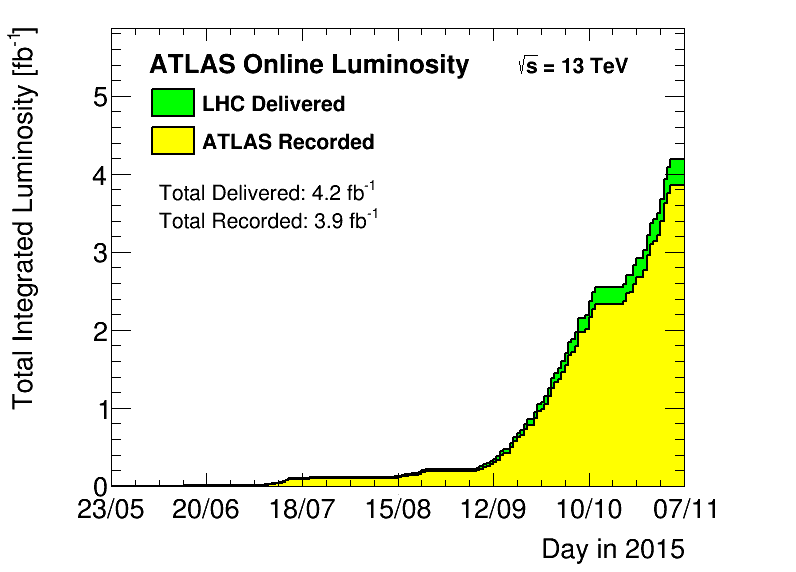
\includegraphics[width=\textwidth]{fig/sumLumiByDay.png}
%      \caption{}
%      \label{fig:data_taking_2015}
%    \end{subfigure}%
%    ~%add desired spacing
%    \begin{subfigure}[b]{0.45\textwidth}
%      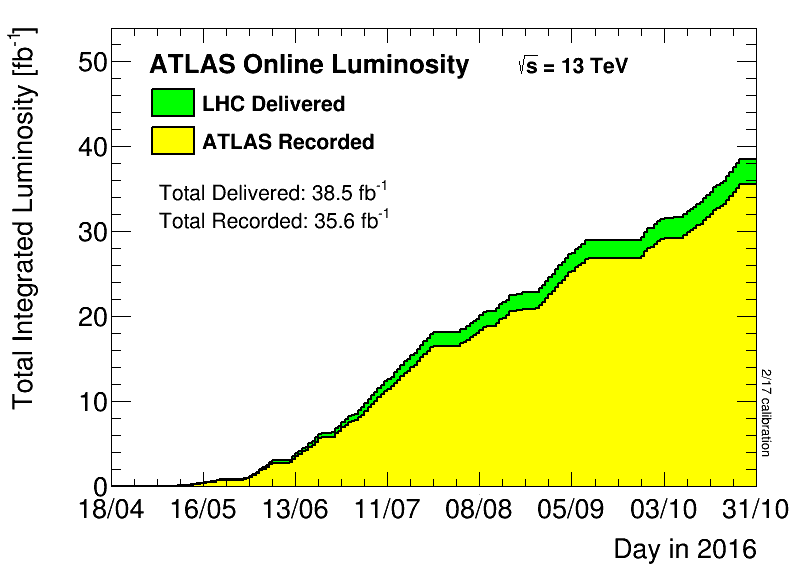
\includegraphics[width=\textwidth]{fig/sumLumiByDay_2016.png}
%      \caption{}
%      \label{fig:data_taking_2016}
%    \end{subfigure}
%    \caption{ATLAS数据收集情况:(a) 2015年,(b) 2016年。}
%    \label{fig:data_taking}
%\end{figure}

%\subsection{蒙特卡罗样本}

\subsection{信号样本}
信号样本包含两种模型,分别为希格斯粒子对($pp\rightarrow (X) \rightarrow hh$)和类希格斯粒子对($gg \rightarrow X \rightarrow SS$)。
%\subsubsection{$gg\rightarrow (X) \rightarrow hh$}
\begin{enumerate}
    \item SM 信号(非共振态模式)目前只考虑胶子融合过程,即$gg\rightarrow hh$,利用包含NLO修正的双希格斯粒子模型~\cite{Frederix:2014hta},
    在\MGMCatNLO~\cite{madgraph5amcnlo,syscalc}中产生。
%其产生截面为33.4 fb~\cite{eftreweight,HiggsXSec},考虑了NNLO QCD修正和including resummation of soft-gluon emission at next-to-next-to-leading-logarithmic (NNLL) accuracy for $m_{H} = 125.09$~GeV。 
    \item 共振态模式($gg\rightarrow X\rightarrow  hh$)利用包含NLO修正的\texttt{2HDMCP\_EFT}的信号模型~\cite{MG5-HH-LO},在\MGMCatNLO 中产生。其中重标量粒子X,即共振态粒子,被假设具有远小于实验精度的衰变宽度;
在实际模拟中,其宽度设为10 MeV,并考虑四个质量点,分别为260 GeV, 300 GeV, 400 GeV和500 GeV。此过程产生截面假设为1 pb。 
\end{enumerate}
两个希格斯粒子均要求衰变到$W$玻色子对,随后,其中两个$W^{+}(W^{-})$衰变到轻子(包括$\tau$),而另两个$W^{-}(W^{+})$则到强子对。这一系列衰变通过\Herwigpp~\cite{herwigpp}实现,也包括随后的部分子簇射和强子化过程,其衰变分支比为$BR(hh\rightarrow 4W \rightarrow \ell^{\pm}\nu\ell^{\pm}qqqq)=4.4\times10^{-3}$。两种模式的信号样本的产生情况总结如表~\ref{tab:dsid_hh}所示。
\begin{table}
\centering
\small
\begin{tabular}{cccccc}
                        \hline
                        \hline
                        DSID & lepton charge & $m_X$ [GeV] & Num. Events & Simulation & e/a/s/r/p-tags\\
                        \hline
                        344133  &$++$  & Non-res &  500000 &  AFII &  e5060, a766, a821, r7676, p2949  \\
                        344134  &$--$ & Non-res &  500000 &  AFII &  e5060, a766, a821, r7676, p2949  \\
                        343704  &$++$ & 260     &  100000 &  AFII &  e5234, a766, a821, r7676, p2949 \\
                        343712  &$--$ & 260     &  100000 &  AFII &  e5234, a766, a821, r7676, p2949 \\
                        343706  &$++$ & 300     &  100000 &  AFII &  e5234, a766, a821, r7676, p2949 \\
                        343714  &$--$ & 300     &  100000 &  AFII &  e5234, a766, a821, r7676, p2949 \\
                        343709  &$++$ & 400     &  100000 &  AFII &  e5153, a766, a821, r7676, p2949 \\
                        343717  &$--$ & 400     &  100000 &  AFII &  e5153, a766, a821, r7676, p2949 \\
                        343711  &$++$ & 500     &  100000 &  AFII &  e5153, a766, a821, r7676, p2949 \\
                        343719  &$--$ & 500     &  100000 &  AFII &  e5234, a766, a821, r7676, p2949 \\
                        \hline
                        \hline
\end{tabular}
\caption{Summary of the MC $hh$ samples which have been produced for study.}
\label{tab:dsid_hh}
\end{table}


%\subsubsection{$gg \rightarrow X \rightarrow SS$}
$gg \rightarrow X \rightarrow SS$利用\PYTHIAV{8}~\cite{pythia8}在LO阶产生,PDF为\texttt{A14NNPDF2.3LO},模型为\texttt{HiggsBSM:gg2A3},X和S均假设具有远小于实验分辨率的宽度,为各自质量的1\%。与$gg\rightarrow (X) \rightarrow hh$类似,S被要求衰变到两个$W$玻色子,其中两个$W^{+}(W^{-})$被要求衰变到轻子(包括$\tau$),而另两个$W^{-}(W^{+})$则到强子对。随后的部分子簇射与强子化过程也由\PYTHIAV{8}实现。$m_X$和$m_S$选择使得4W 末态能够最显著。同样的,$gg \rightarrow X \rightarrow SS$截面假设为1 pb,而$BR(S\rightarrow WW)$则依赖于$m_S$,即希格斯粒子在不同质量点的衰变分支比~\cite{Denner:2011mq}。
表~\ref{tab:dsid_SS}总结了此信号样本产生情况。
\begin{table}[!htbp]
  \centering
  \begin{tabular}{c c c c r r}
    \hline
    \hline
    %\toprule
    Charge & $m_X$ & $m_S$ & BR$(\text{two SS leptons})$ & DSID & $N_{\text{events}}$ \\
    %\midrule
    \hline
    \multirow{7}{*}{$++$} & 280 GeV & 135 GeV & $1.47\times10^{-2}$ &344927  & 25000 \\
     & 300 GeV & 135 GeV & $1.535\times10^{-2}$ &344928  & 25000 \\
     & 320 GeV & 135 GeV & $1.535\times10^{-2}$ &344930  & 25000 \\
     & 340 GeV & 135 GeV & $1.535\times10^{-2}$ &344933  & 25000 \\
     & 340 GeV & 145 GeV & $3.454\times10^{-2}$ &344934  & 25000 \\
     & 340 GeV & 155 GeV & $6.049\times10^{-2}$ &344935  & 24000 \\
     & 340 GeV & 165 GeV & $8.842\times10^{-2}$ &344936  & 25000 \\
    \hline
    %\midrule
    \multirow{7}{*}{$--$} & 280 GeV & 135 GeV & $1.47\times10^{-2}$ &344937  & 25000 \\
     & 300 GeV & 135 GeV & $1.535\times10^{-2}$ &344938  & 25000 \\
     & 320 GeV & 135 GeV & $1.535\times10^{-2}$ &344940  & 25000 \\
     & 340 GeV & 135 GeV & $1.535\times10^{-2}$ &344943  & 25000 \\
     & 340 GeV & 145 GeV & $3.454\times10^{-2}$ &344944  & 24000 \\
     & 340 GeV & 155 GeV & $6.049\times10^{-2}$ &344945  & 25000 \\
     & 340 GeV & 165 GeV & $8.842\times10^{-2}$ &344946  & 25000 \\
    \hline
    \hline
    %\bottomrule
  \end{tabular}
  %\caption{Summary of the MC $X\rightarrow SS$ signal samples used.}
  \caption{$X\rightarrow SS$ MC产生总结,每个质量包含$++(\ell^+\ell^+)$与$--(\ell^-\ell^-)$,分支比$BR$对应
$pp\rightarrow X\rightarrow SS\rightarrow \ell^{\pm}\ell^{\pm}qqqq$。}
  \label{tab:dsid_SS}
\end{table}


\subsection{背景样本}
多玻色子(VV/VVV)和$V\gamma$样本通过\SHERPAV{2.1}~\cite{sherpa}在NLO阶产生;$V+jets$则通过\SHERPAV{2.2}在NLO阶产生,此两种过程均采用CT10 PDF。$VH$利用\PYTHIAV{8}在LO阶产生,采用NNPDF2.3LO PDF。$t\bar{t}$通过\POWHEGBOXV{2.0}~\cite{powhegbox}在NLO阶产生,而后传递到\PYTHIAV{8}进行部分子簇射和强子化模拟,采用PDF为NNPDF2.3LO。单顶夸克过程($t+X$)同样通过\POWHEGBOXV{2.0}在NLO阶产生,但传递到\PYTHIAV{6.4}~\cite{pythia6}进行后续模拟,采用PDF则为CT10。$t\bar{t}V$样本则在NLO阶通过\MGMCatNLO+\PYTHIAV{8}产生,采用PDF为NNPDF2.3LO。$t\bar{t}H$样本通过\MGMCatNLO+\Herwigpp 产生,PDF为NNPDF3.0~\cite{PDF:NNPDF30}。更多关于这些背景过程的产生及模拟过程可参考文献~\cite{ATL-PHYS-PUB-2016-004,ATL-PHYS-PUB-2016-005,ATL-PHYS-PUB-2016-002}。

